\documentclass[a4paper,14pt]{extarticle}
\def\source{/home/osabio/tex/templates}
\input{\source/head.tex}
\irodov{3.65}{Электростатика}
% Стыдить лжеца, шутить над дураком
% И спорить с женщиной — всё то же,
% Что черпать воду решетом:
% От сих троих избавь нас, боже!..

% М. Ю. Лермонтов.
\begin{document}

\begin{figure}[H]
    \centering
    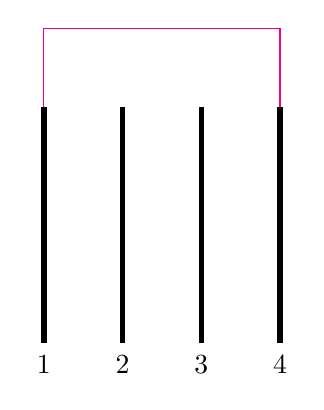
\begin{tikzpicture}
        \draw[line width=2pt] (0,0) node[below] {$1$} -- ++(0,3);
        \draw[line width=2pt] (1,0) node[below] {$2$} -- ++(0,3);
        \draw[line width=2pt] (2,0) node[below] {$3$} -- ++(0,3);
        \draw[line width=2pt] (3,0) node[below] {$4$} -- ++(0,3);

        \draw[magenta] (0,3) -- (0,4) -- (3,4) -- (3,3);
    \end{tikzpicture} 
\end{figure}
% \begin{equation}
% 	\phi_1-\phi_4=(\phi_1-\phi_2)+(\phi_2-\phi_3)+(\phi_3-\phi_4)=(\phi_1-\phi_2)+\Delta\phi+(\phi_3-\phi_4)=0
% \end{equation}
% Откуда
% \begin{equation}
% 	(\phi_1-\phi_2)+(\phi_3-\phi_4)=-\Delta\phi
% \end{equation}
Считаем, что на пластине $3$ $\sigma_3>0$, тогда на пластине $2$ $\sigma_2=-\sigma_3$.

На пластинах $1$ и $3$ индуцируются заряды: тогда 
\begin{equation}
	\sigma_1=-\sigma_4
\end{equation}
из закона сохранения зарядов.

Внутреннее поле между пластинами $2$ и $3$:
\begin{equation}
	E_{23}^{in}=2\pi\sigma_2-2\pi\sigma_3=4\pi\sigma_2
\end{equation}
Внешнее поле обеспечивается индуцированным зарядом между $1$ и $4$:
\begin{equation}
	E_{23}^{ext}=2\pi\sigma_4-2\pi\sigma_1=4\pi\sigma_4
\end{equation}
% Тогда поля между парами пластин:
\begin{equation}
	E_{12}=E_{34}=E_{23}^{ext}=4\pi\sigma_4
\end{equation}
\begin{equation}
	E_{23}=E_{23}^{in}-E_{23}^{ext}=4\pi(\sigma_2-\sigma_4)
\end{equation}
% Так как расстояние между пластинами мало, то
\begin{equation}
	\Delta\phi=E_{23}d \quad\Rightarrow\quad E_{23}=\frac{\Delta\phi}{d}
\end{equation}
% Из условия замкнутости
\begin{equation}
	\phi_1-\phi_4=-E_{12}d+E_{23}d-E_{34}d=0
\end{equation}
% Откуда
\begin{equation}
	E_{12}=E_{34}=E_{23}^{ext}=\frac12E_{23}=\frac{\Delta\phi}{2d}
\end{equation}
\begin{equation}
	E_{23}^{in}=E_{23}-E_{23}^{ext}=\frac{3\Delta\phi}{2d}
\end{equation}
Тогда
\begin{equation}
	-\sigma_1=\sigma_4=\frac{E_{23}^{ext}}{4\pi}=\frac{\Delta\phi}{8\pi d}
\end{equation}
\begin{equation}
	-\sigma_3=\sigma_2=\frac{E_{23}^{in}}{4\pi}=\frac{3\Delta\phi}{8\pi d}
\end{equation}

\end{document}